\chapter{Base Model For Crime Inference}



\section{Problem Formulation}

\label{sec:problem-formulation}
The crime dataset in Chicago has detailed information about the time and location (i.e., latitude and longitude) of crime and the types of crime. In our problem, when we use term crime count, we often refer to crime count in a  region (i.e., community area) in a year. The \emph{community area} is used as our geographical unit of study, since it is well-defined,  historically recognized and stable over time~\cite{wiki-ca}. In total, there are 77 community areas in Chicago.  Crime rate is the crime count normalized by the population in a region. We use vector $\vec{y} = [y_1, y_2, \ldots, y_n]$ to denote the crime rate in region $i$. The crime rate inference problem is to estimate the crime rate in one region using the crime rate of other regions in the same year by considering the features of regions and correlations between regions. 


The crime data of Chicago are obtained from City of Chicago data portal~\cite{crime-data}. Chicago is the city with most complete crime data that are made public online. The crime dataset contains the incident date, location (strict name and GPS coordinates), and primary type from year 2001 to 2015. In total there are $5,856,414$ recorded crime incidents over 15 years, which is an average $390,417$ crimes incidents per year. We visualize the crime normalized by population in Figure~\ref{fig:crime-ca}, from which we can see that the downtown area has the highest crime rate.

\begin{figure}[t]
\centering
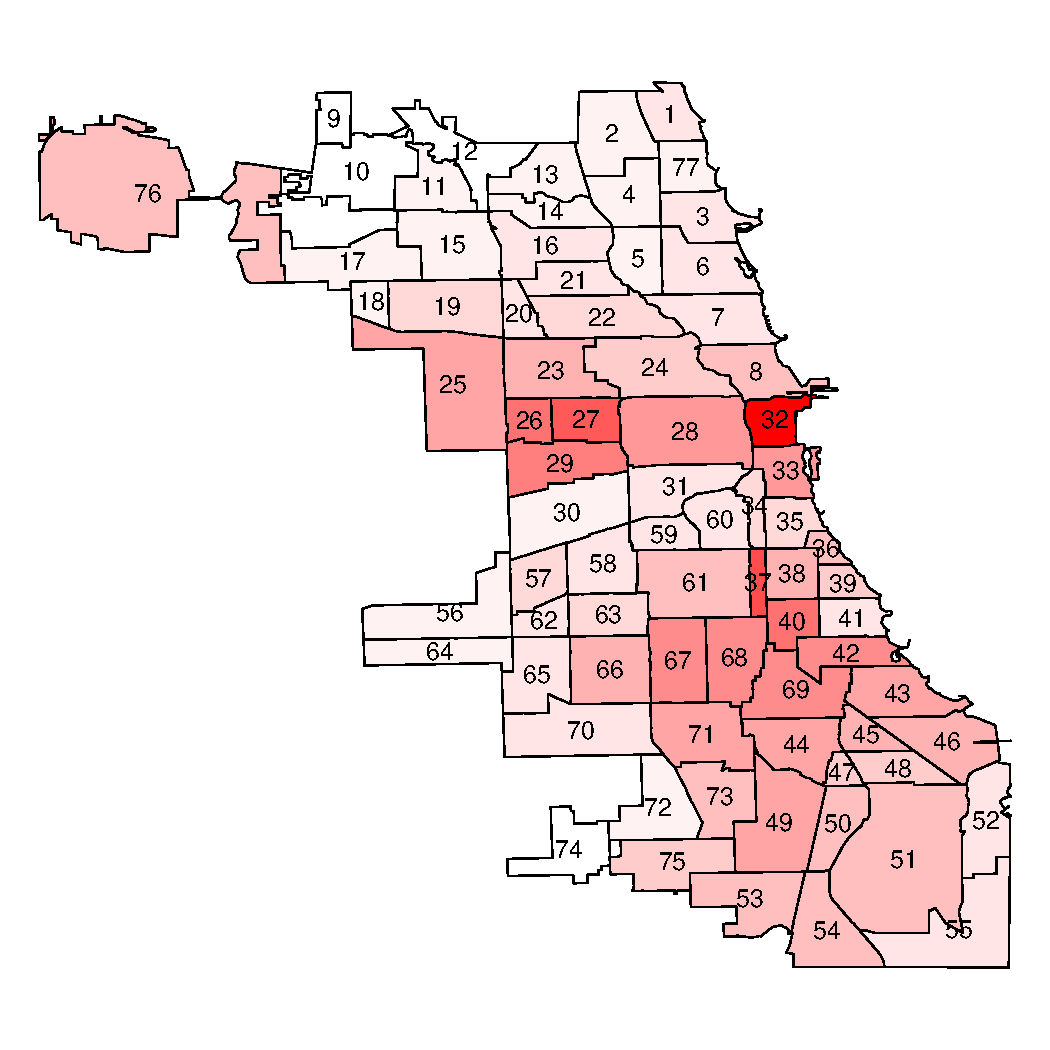
\includegraphics[width=0.7\textwidth]{fig/crime-ca.pdf}
\caption{Crime rate of Chicago by community areas. The community area \#32 is Chicago downtown, which has the highest crime rate.}
\label{fig:crime-ca}
\end{figure}


In this paper we study the crime rate inference problem. More specifically, we estimate the crime rate of some regions given the information of all the other regions. Without loss of generality, we assume there is one community area $t$ with crime rate $y_t$ missing, and we use the crime rate of all the other regions $\{y_i \} \backslash y_t$ to infer this missing value. Our problem is mathematically formalized as follows
\begin{equation}
\hat{y_t} = f( \{y_i\} \backslash y_t, X),
\end{equation}
where  $X$ refers to observed extra information of  all those community areas.




\smallskip
We consider two  types of features $X$ for inference:
\begin{itemize}
\item Nodal feature. Nodal features describe the characteristics of the focal region. Such features include demographic information and Point-of-Interest (POI) distribution. Demographics are frequently used in literature, but POI is a newer type of big data, which we find significantly improve the crime inference accuracy.
\item Edge feature: (1) Geographical influence. Geographical influence considers the crime rate of the nearby locations.  This feature has been extensively used in
literature as well. To estimate the focal region, the
crime rate of nearby regions are weighted according
to spatial distances. (2) Hyperlink by taxi flow. Locations are connected through the frequent trips made by humans, which can be considered as the hyperlinks in space. This type of feature has never been studied in literature. We propose to use taxi trips to construct the social flow. Our hypothesis is that similarity in the crime rate of two regions should correlate with the social flow strength between these two regions. 
\end{itemize}





\section{Base Inference Model}



\subsection{Linear Regression}
The most straightforward prediction is linear regression model. This model assumes the error terms follow a Gaussian distribution $\epsilon \sim \mathcal{N}(0, \sigma^2)$. As a result the parameter distribution also follows a Gaussian distribution. This assumption makes the model less generative, since in real applications, there is no way to ensure the dependent variable has a Gaussian error term. 


Equation~\ref{eq:lrm} gives the linear regression formulation of our problem.
\begin{equation}
\label{eq:lrm}
\vec{y} = \vec{\alpha}^T \vec{x} + \beta^f W^f \vec{y} + \beta^g W^g \vec{y} + \vec{\epsilon},
\end{equation}
where $\vec{x}$ represents the nodal features including demographics and POI distribution, $W^f$ is the flow matrix of taxi flow, and $W^g$ is the spatial matrix representing the geographical adjacency. On the right-hand side, $\epsilon$ is the only stochastic variables, and all other terms are fixed observation values. Therefore, we incorporate all the fixed observations into one term $X$, and we get the standard regression problem
\[
E(y) = X w + \epsilon.
\]


In order to learn the regression parameter $w$, we can use a maximum likelihood estimator. Since $\epsilon = y - Xw$, the joint probability of error term is
\begin{equation}
P(\epsilon | w) = \frac{1}{\sqrt{2\pi \sigma^2}} e^{-\frac{(y - Xw)^2}{2 \sigma^2}}.
\end{equation}
Maximizing the joint probability gives us the optimal solution.






\section{Feature Extraction}
\label{sec:feature}


In this section, we will discuss the details of features used in our method. The two types of new features we will use are extracted from Point-Of-Interest data and taxi flow data. Below we will describe the datasets used to construct features and the characteristics of these features.

\begin{figure*}[t]
\centering
\subfigure[Total population]{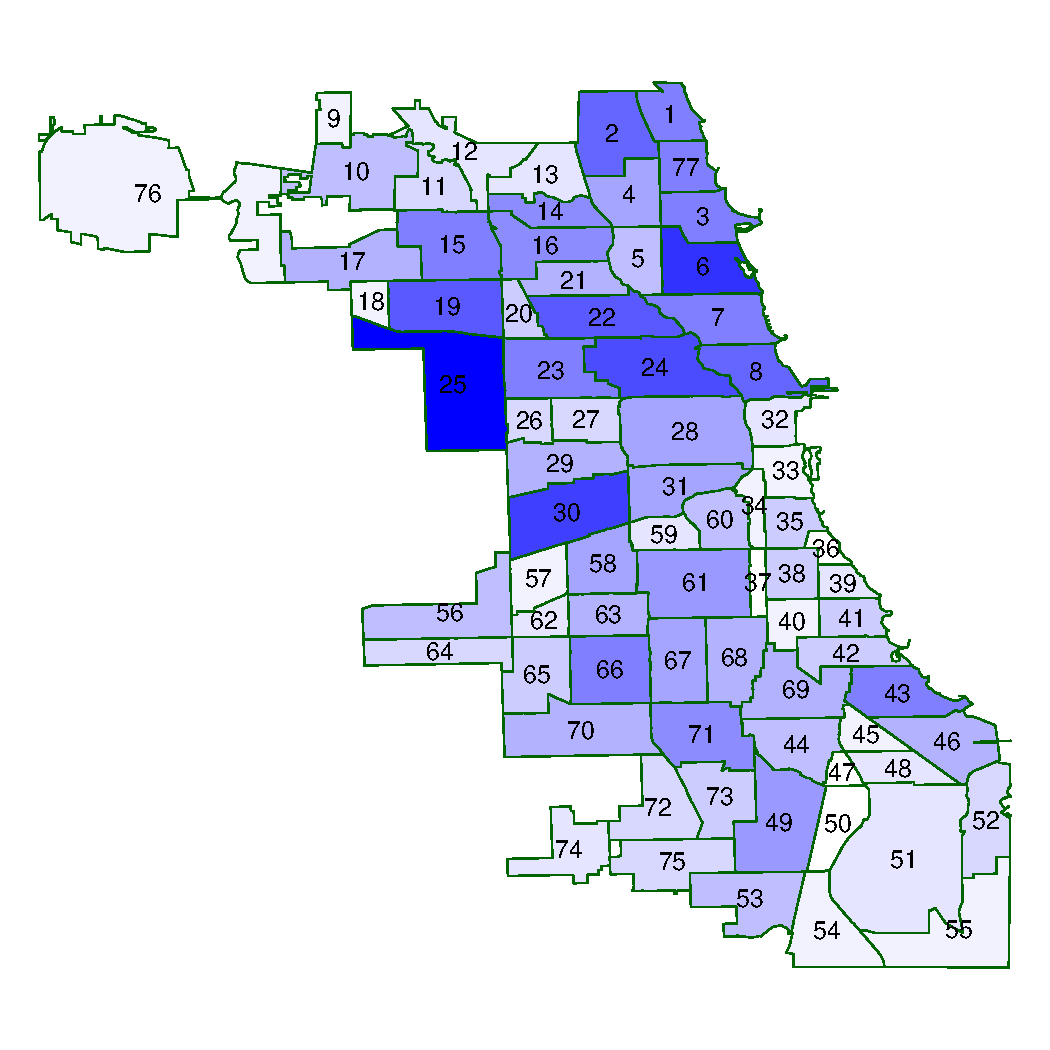
\includegraphics[width=0.45\textwidth]{fig/demo-f1.pdf}}
\subfigure[Poverty index]{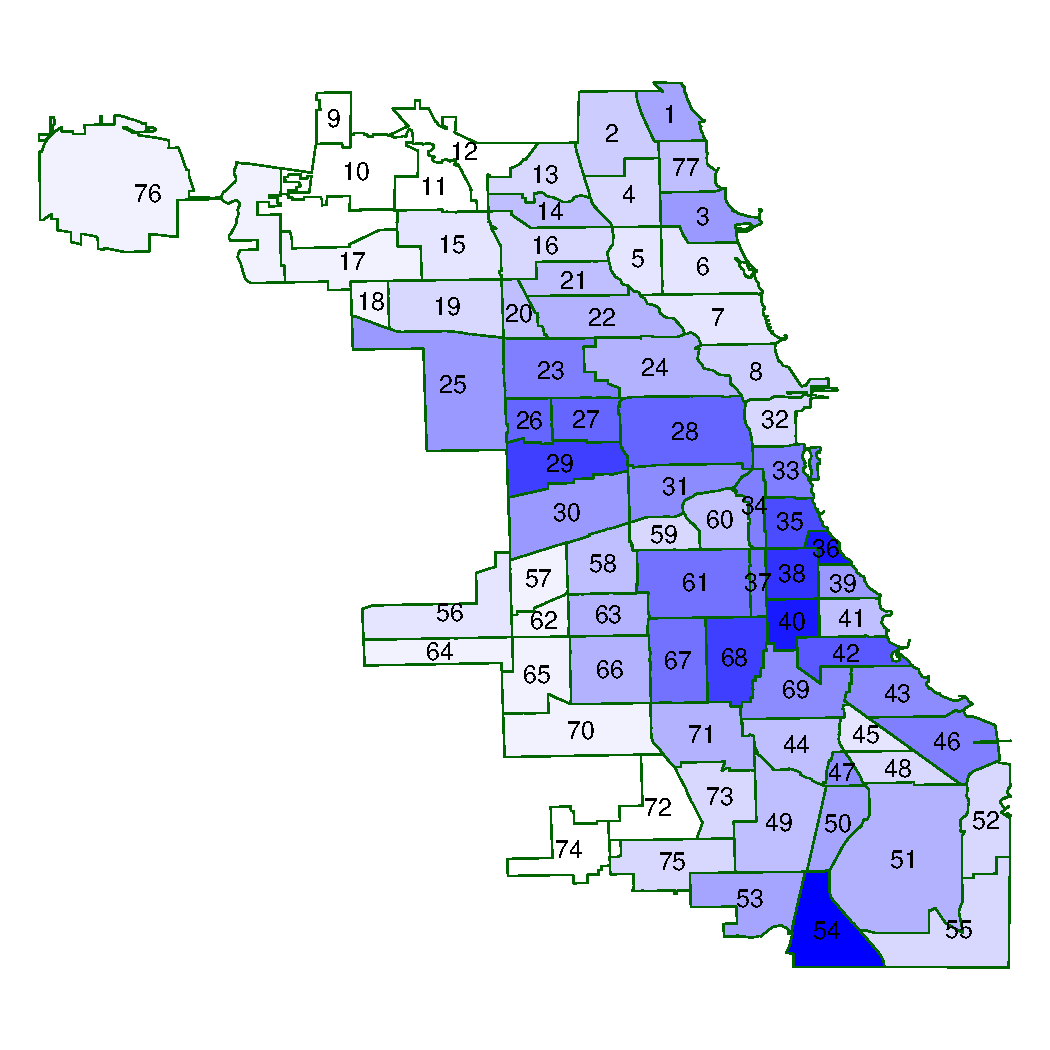
\includegraphics[width=0.45\textwidth]{fig/demo-f3.pdf}}
\subfigure[Disadvantage index]{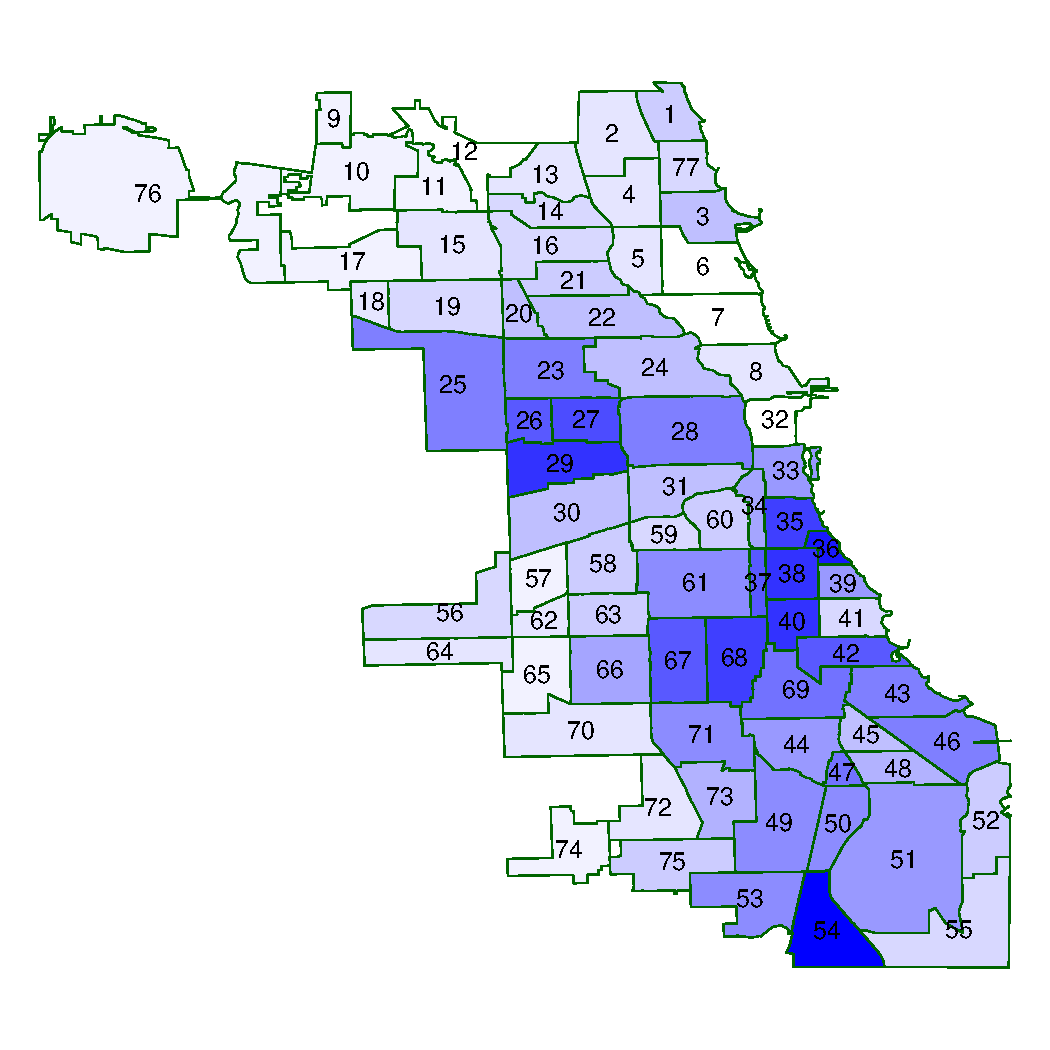
\includegraphics[width=0.45\textwidth]{fig/demo-f4.pdf}}
\subfigure[Ethnic diversity]{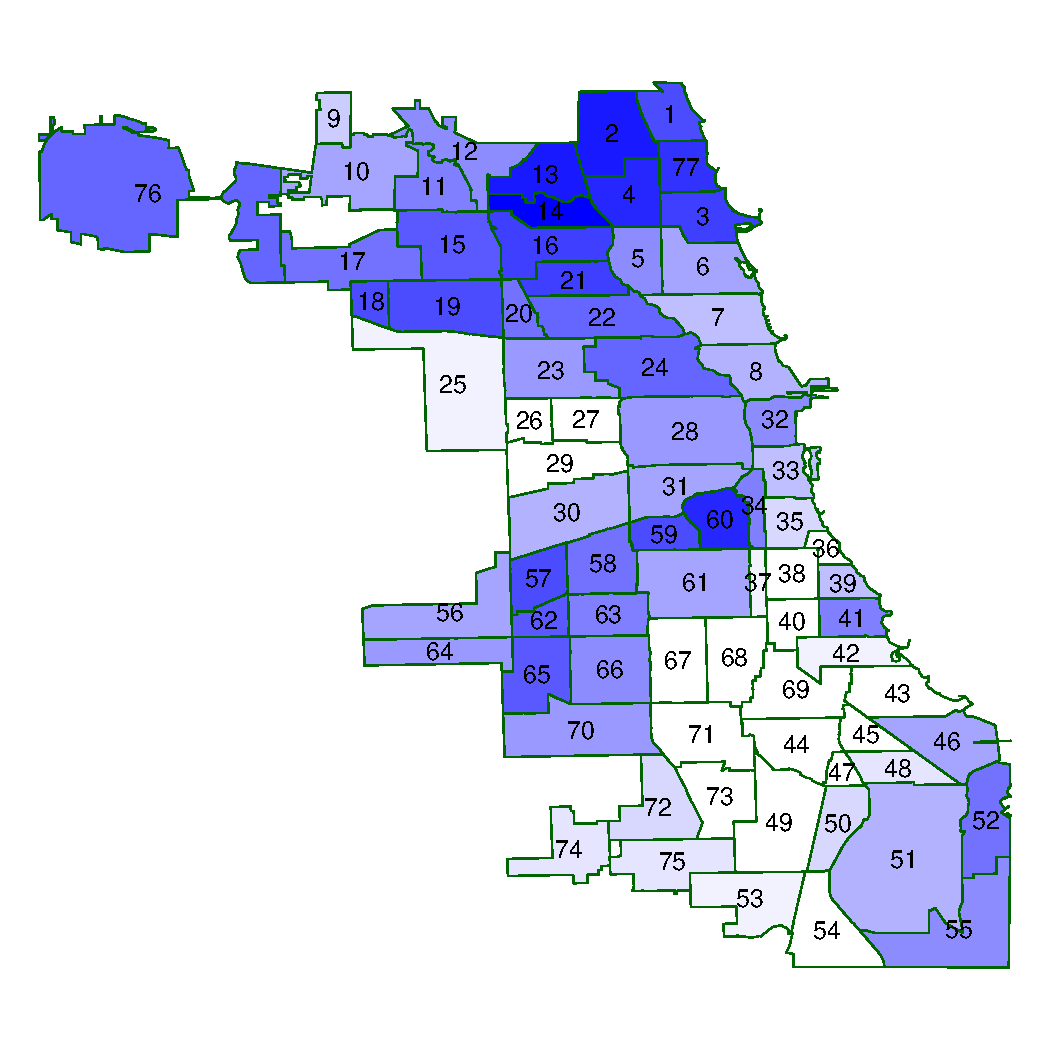
\includegraphics[width=0.45\textwidth]{fig/demo-f6.pdf}}
\caption{(a)-(d) Demographics in Chicago by community areas. Darker colors indicate higher values.}
\label{fig:demo-f}
\end{figure*}





\subsection{Nodal Feature: Demographics}

Socioeconomic and demographic features of neighborhoods have been
widely used to predict crime~\cite{Bogo14, HsPu93, WoMe12, SaHi07}. Previous studies have shown that crime rate correlates with certain demographics. For example, \cite{Jac61, GrSa09} suggests that population diversity leads to less crime in certain neighborhoods. 
In our study, we include demographic information from the US Census Bureau's Decennial Census of 2010~\cite{census-data} and American Community Survey's five-year average estimates
between 2007 and 2011. We use year 2010 data because we are evaluating crime rates in 2010-2013. The demographics include the following features:

\textsf{total population, population density, poverty, disadvantage index, residential stability, ethnic diversity, race distribution}.


The poverty index measures the proportion of community area residents
with income below the poverty level. The disadvantage index is
a composite scale based on prior work \cite{SRE97}, a function of 
poverty, unemployment rate, proportions of families with public
assistance income, and proportion of female headed households. 
 The residential stability measures home ownership and proportion of
residents who lived in the neighborhood for more than one year. Racial
and ethnic diversity is an index of heterogeneity~\cite{GrSa09} based on six
population groups, including: Hispanics, non-Hispanic Blacks, Whites,
Asians, Pacific Islanders and others.


Figure~\ref{fig:demo-f} visualizes the crime rate and demographics features in Chicago by community areas. Comparing with Figure~\ref{fig:crime-ca}, it is clear that the crime rate and poverty index and disadvantage index are consistent,  the ethnic diversity shows an inverse correlation, and the total population has little correlation with crime.



Table~\ref{tb:demo} shows the Pearson correlation coefficient between various demographics features and the crime rate at community area level. The corresponding p-value is also calculated and shown in the table to indicate the significance of the correlation coefficient.  There  are in total $77$  community areas in Chicago. Table~\ref{tb:demo} shows such correlation with several most correlated features. We can see that the poverty index and disadvantage index positively and strongly correlate with crime, while the ethnic diversity negatively correlates with crime. Other features such as total population, population density, and residential stability  have weaker correlations. One counter-intuitive observation is that the total population has a weak and negative correlation with crime. The reason is that we use crime rate in each community area, which is already normalized by the population, and therefore the total population and population density have less impact. 


\begin{table}[h]
\centering
\caption{Pearson correlation between demographic features  and crime rate (\textbf{*} indicates significant correlations with p-value less than $5\%$). }
\vspace{2mm}
\begin{tabular}{|c||c|c|}
\hline
Feature & Correlation & p-value \\ \hline \hline
Total Population & -0.1269 &  0.2716 \\ \hline
Population Density & -0.1972  & 0.0855 \\ \hline
Poverty Index & \textbf{0.5573*} & 1.403e-07 \\ \hline
Disadvantage Index & \textbf{0.5959*} & 1.082e-08 \\ \hline
Residential Stability  & -0.0453 &  0.6965 \\ \hline
Ethnic Diversity & \textbf{-0.5545*} &  1.678e-07 \\ \hline
Percentage of Black & \textbf{0.6696*} &  2.779e-11 \\ \hline
Percentage of Hispanic  & \textbf{-0.3820*} &  0.0006 \\ \hline
\end{tabular}
\label{tb:demo}

\end{table}







\subsection{Nodal Feature: Point-of-Interest (POI)}

While demographics are traditional census data, POI is a type of  modern data that provide fine-grained information about locations. We collect POI from FourSquare~\cite{poi-data}. POI data from FourSquare provide the venue information including venue name, category, number of check-ins, and number of unique visitors. We mainly use the major category information because categories can characterize the neighborhood functions. There are 10 major categories defined by FourSquare:

\textsf{food, residence, travel, arts \& entertainment, outdoors \& recreation, college \& education, nightlife, professional, shops, and event.}


\begin{figure}[tb]
\centering
\subfigure[Nightlife]{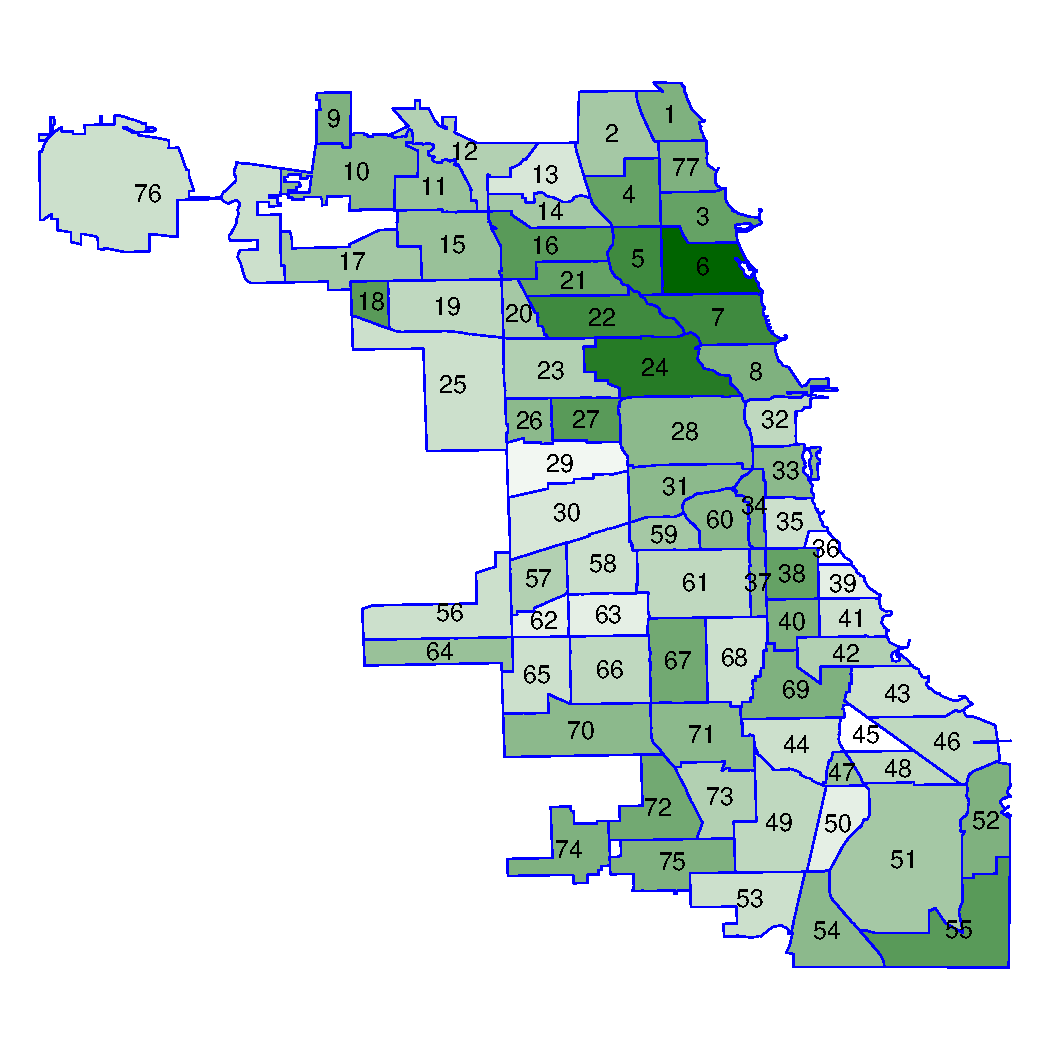
\includegraphics[width=0.45\textwidth]{fig/poi-dist7.pdf}}
\subfigure[Professional]{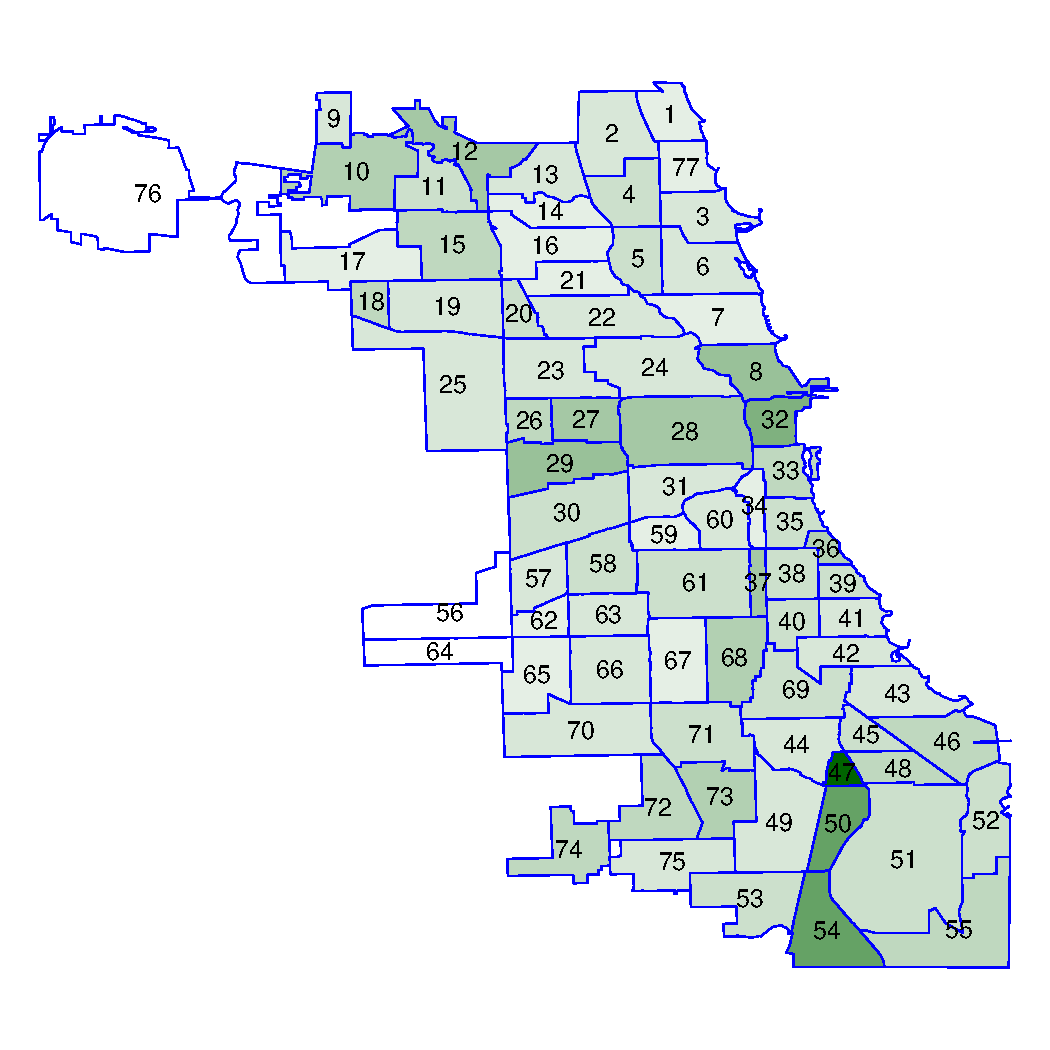
\includegraphics[width=0.45\textwidth]{fig/poi-dist8.pdf}}
\caption{Plot the  POI ratio per neighborhood. The saturation of color is proportional to the ratio value. The ``professional'' category distribution is more consistent with the crime distribution, and therefore it is the most correlated with crime. Meanwhile, the ``nightlife'' category is not positively correlated with Chicago crime.}
\label{fig:poi-coef}
\end{figure}

In total, we have crawled $112,000$  POIs from FourSquare for Chicago. Most of these POIs are in downtown area of Chicago. We normalize the POIs count per category by the total POI count in a neighborhood and plot two selected category, i.e. nightlife and professional, in Figure~\ref{fig:poi-coef}.  The darker colored neighborhoods in Figure~\ref{fig:poi-coef} are the ones with a higher portion of residence POIs.



\begin{table}[h]
\centering
\caption{Pearson correlation between POI category and crime rate (\textbf{*} indicates significant correlations with p-value less than $5\%$).}
\vspace{2mm}

\label{tb:poi-corr}
\begin{tabular}{|c ||c|c|}
\hline
POI category & Correlation & p-value \\ \hline \hline
Food & -0.1543 &  0.1803 \\ \hline
Residence &  -0.0610 &  0.5984 \\ \hline
Travel & -0.0017 &  0.9883 \\ \hline
Arts \& Entertainment & -0.0049 &  0.9661 \\ \hline
Outdoors \& Recreation &  0.0668 &  0.5637 \\ \hline
College \& Education & -0.0078 &  0.9473 \\ \hline
Nightlife &  -0.1553 &  0.1775 \\ \hline
Professional & \textbf{0.3221*} &  0.0043 \\ \hline
Shops & -0.1676 &  0.1450 \\ \hline
Event & 0.2196 &  0.0549  \\ \hline
\end{tabular}
\end{table}



In Table~\ref{tb:poi-corr} we show the Pearson correlation between POI category and crime rate. The category ``professional''  is most significantly correlated with the crime rate. Under the professional POI category, there are some venues with a large population concentration, such as transportation center, convention center, community center, and coworking space. In those venues, the  population volume is high and residential stability is low, therefore the professional POI counts positively correlates with crime rate.  One counter-intuitive observation is that ``nightlife'' category is not positively correlated with crime ($-0.1553$). This can be explained through Figure~\ref{fig:poi-coef}(a). The majority of nightlife venues in Chicago locate in northern area, while most crime incidents occur in downtown area.








\subsection{Edge: Geographical Influence}

Together with the US census demographics data, we also collected the boundary shape files of Chicago, which are used to calculate the geographical influence feature.

Previous studies have also shown that the crime rate at one location is highly correlated with nearby locations~\cite{GSGL01, Bur88}. Such geographical influence is also frequently used in the literature~\cite{ACC00, MoSa97}, which is calculated as:
\begin{equation}
\vec{F^g} = W^g \cdot \vec{Y},
\label{eq:spatial}
\end{equation}
where $W^g$ is the spatial weight matrix. If region $i$ and $j$ are not geospatially adjacent, $w_{ij}^g = 0$; otherwise, $w_{ij}^g \propto distance(i,j)^{-1}$.

\begin{figure}[t]
\centering
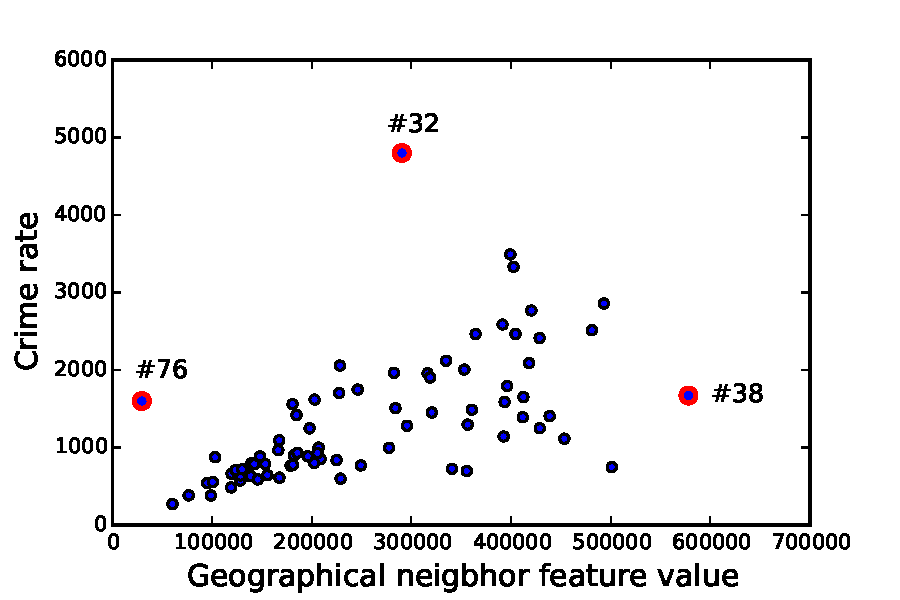
\includegraphics[width=0.8\textwidth]{fig/spatial-crime-rate.pdf}
\caption{The geographical influence feature correlation with crime. In the plot we marked out three outliers and their corresponding community area ID.}
\label{fig:spatial}
\end{figure}

In Figure~\ref{fig:spatial},  we plot crime rate with respect to geographical influence calculated in Eq.~\ref{eq:spatial}. We observe an obvious positive correlation, which means if nearby neighborhoods have a high crime rate, the focal neighborhood is more likely to have a high crime rate. We also do observe a few outliers in Figure~\ref{fig:spatial}. These neighborhoods show different crime rate in their nearby neighborhoods compared to their own. For example, as we can also see in Figure~\ref{fig:crime-ca}, community area \#38 locates in an area where the the neighbors have high crime rates but its crime rate is relatively low; in contrast, neighborhood \#32 has a high crime rate even though its neighbors have relatively low crime. The community area \#76 home of the O'Hare International Airport is far from most of other community areas, however its own crime rate is relative high.









\subsection{Edge: Hyperlinks by Taxi Flow}

In our Chicago taxi dataset, there are $1,048,576$ taxi trips in total during the October to December in 2013. For each trip the following information are available: pickup/dropoff time, pickup/dropoff location, operation time, and total amount paid. We requested the taxi trip records from Chicago taxi commission pursuant of the Freedom of Information Law.  Figure~\ref{fig:taxi-flow} shows a visualization of the major flows at community level.

\begin{figure}[htb]
\centering
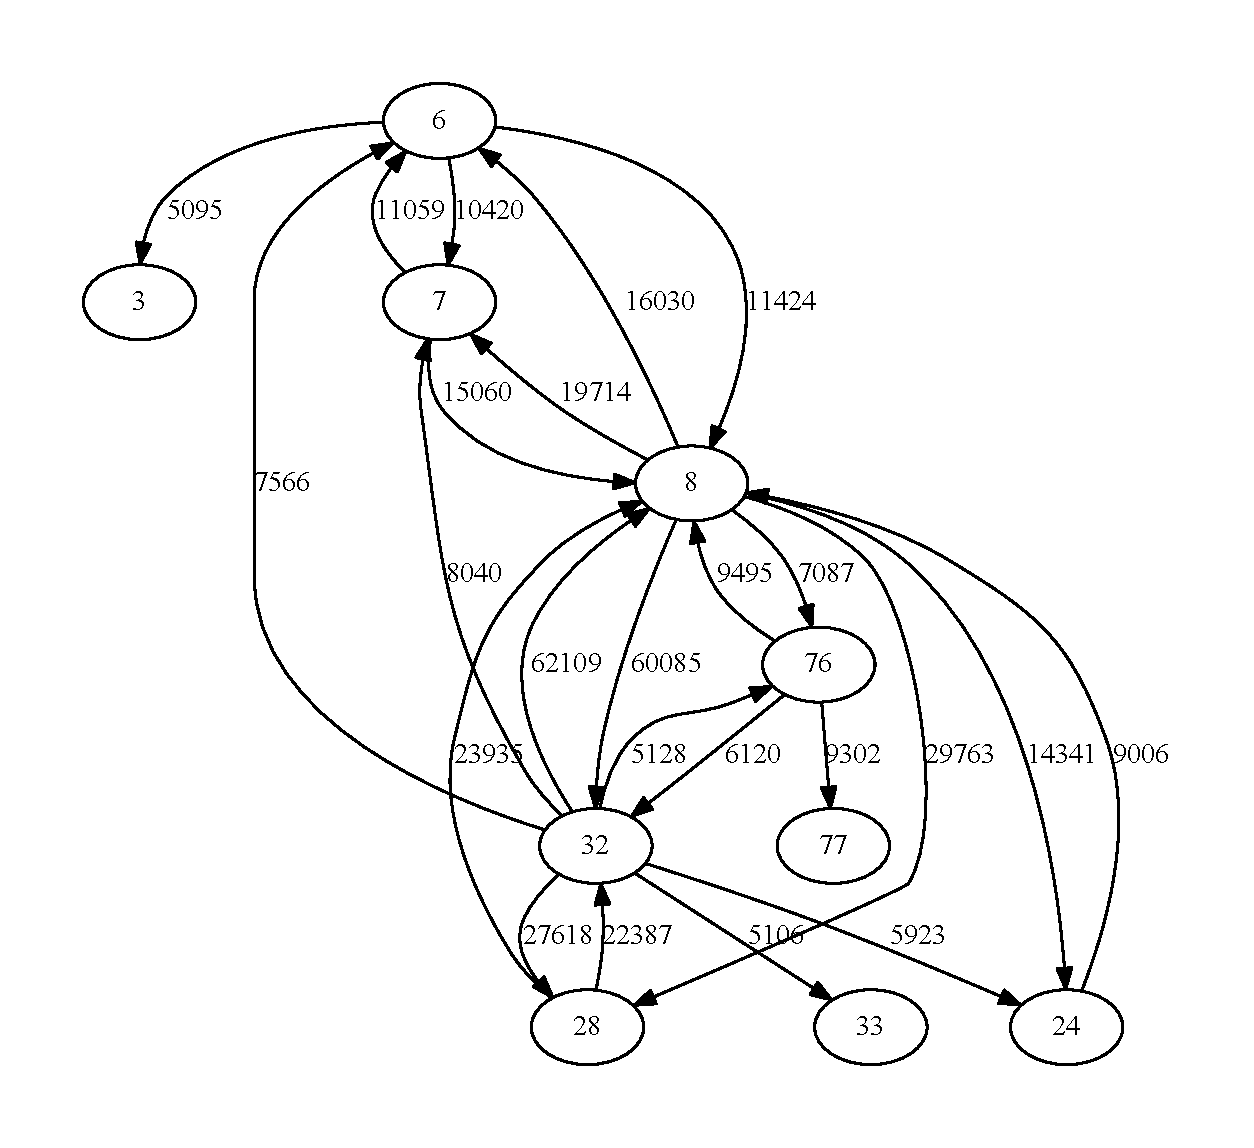
\includegraphics[width=0.8\textwidth]{fig/taxiflow.pdf}
\caption{Major taxi flows between neighborhoods. We set a threshold ($> 5,000$) on the flow and only plot the high volume flow. The label on the node is the ID of the corresponding community areas. We can see that there are several hub community areas, such as \#6, \#8, \#32, which are all in the downtown areas. The label on the edge shows how many taxi trips are commuting through the two community areas for three months in 2013.}
\label{fig:taxi-flow}
\end{figure}


One of our hypothesis is that the social interaction among two community areas propagates crime from one region to another.
The Chicago taxi data captures the social interactions among various community areas. To calculate this first, we first map all taxi trips to community areas to get the taxi flow $w_{ij}\ \forall i,j \in \{1, 2, \cdots n\}$. Then the taxi flow lag is constructed by the product of social flow and the crime rate of neighboring regions as follows
\begin{equation}
\vec{F^t} = W^t \cdot \vec{Y}.
\label{eq:taxi}
\end{equation}
The taxi flow $W^t$ is a matrix with entry $w_{ij}$ denoting the taxi flow from $i$ to $j$. Note that $\forall i$, $w^s_{ii} = 0$ in matrix $W^t$, because we have to exclude the crime in focal area from its own predictor. The semantic of this taxi flow feature is how many crime in the focal area is contributed by its neighboring areas through social interaction.

The correlation between taxi flow and crime rate is shown in Figure~\ref{fig:taxi-corr}. From the scatter plot, we can see that overall the crime rate is positively correlate with the taxi flow. There are two  outliers clearly shown in Figure~\ref{fig:taxi-corr}. The community area \#32 is the downtown Loop, which has the highest crime rate and is hard to predict by taxi flow. Another anomalous community area \#47 has relatively low crime rate by itself. However, this area has a lot of in flows from high-crime communities. 




\begin{figure}[ht]
\centering
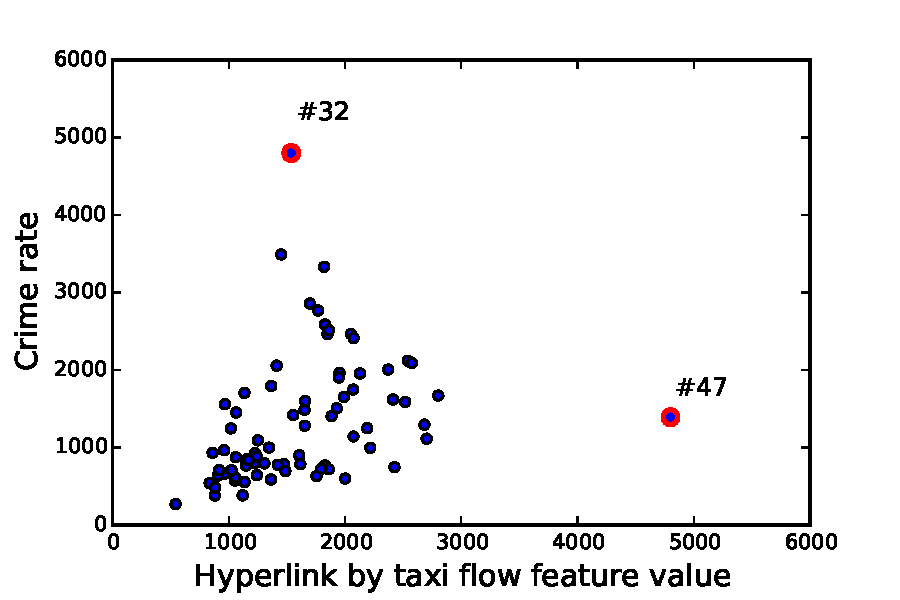
\includegraphics[width=0.8\textwidth]{fig/taxi-flow-percent.pdf}
\caption{Correlation between taxi flow and crime rate. In the plot, we marked out three outliers and their corresponding community area ID.}
\label{fig:taxi-corr}
\end{figure}





\section{Evaluation of Base Model}


We evaluate the linear regression base model. We use a incremental settings, where new features are added on top of previous one. The results are shown in Figure~\ref{fig:lrresult}.


\begin{figure}[h]
\centering
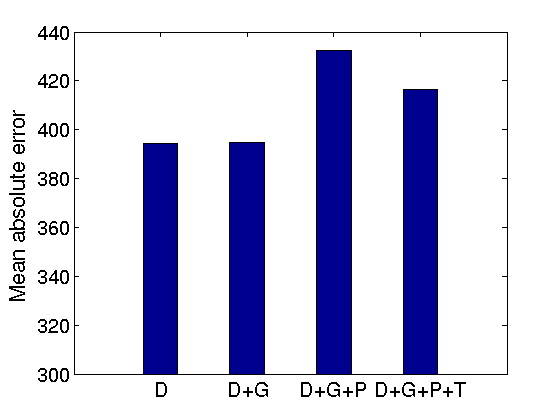
\includegraphics[width=0.8\textwidth]{fig/lrresult.png}
\caption{The inference error for linear regression base model. $^*$D -- demographic features, G -- geographical influence, P -- POI features, T -- taxi flow feature}
\label{fig:lrresult}
\end{figure}


From the result in Figure~\ref{fig:lrresult}, we found that the newly added feature does not improve the inference accuracy. This result is counterintuitive. Dose this mean our intuition is not correct? Or it means that we did not pick the right model.  In the next chapter, we will go into the weakness of the base model. At the same time, we propose some new technique to improve the base model.
